\begin{quote}
\itshape
Na początku był Chaos. Któż zdoła powiedzieć dokładnie, 
co to był Chaos?  
Niejedni widzieli w nim jakąś istotę boską, ale bez określonego kształtu. 
Inni – a takich było więcej – mówili, że to wielka otchłań, pełna siły 
twórczej i boskich nasieni, jakby jedna masa nieuporządkowana, ciężka i ciemna, 
mieszanina ziemi, wody, ognia i powietrza.

\hfill--- Jan Parandowski, \textit{Mitologia Grecka i Rzymska}
\end{quote}
\vspace{1.5em}

Pojęcie chaosu, pierwotnie kojarzone z mitologiczną lub filozoficzną istotą pozbawioną formy, we współczesnej nauce zyskało precyzyjną definicję, przy czym największe znaczenie przypisuje się mu w fizyce oraz matematyce w kontekście nieliniowych układów dynamicznych. Opisywane układy charakteryzują się znaczną wrażliwością na warunki początkowe, w wyniku czego nawet minimalne zmiany parametrów startowych prowadzą do drastycznie odmiennych wyników końcowych, które to zjawisko określa się powszechnie mianem efektu motyla~\cite{motyl2}.
 
Skomplikowana natura zjawisk chaotycznych wymaga stosowania zaawansowanych narzędzi analitycznych, niezbędnych do dokładnego badania oraz modelowania procesów, w związku z czym w dalszej części pracy zaprezentowano podstawy teoretyczne obejmujące metody pomiaru nieuporządkowania oraz sposoby symulowania układów chaotycznych przy użyciu algorytmów uczenia maszynowego.
 
\section{Odwzorowanie logistyczne i geometria fraktalna}
 
Analiza zjawisk chaotycznych w literaturze naukowej jest często rozpoczynana od badania elementarnych, jednowymiarowych modeli dyskretnych, wśród których klasycznym przykładem pozostaje odwzorowanie logistyczne, opisywane nieliniowym równaniem różnicowym. Analiza zachowania tego układu pozwala na ukazanie mechanizmu kaskady bifurkacji, polegającego na tym, że wraz ze wzrostem parametru sterującego początkowo stabilne i przewidywalne rozwiązania zaczynają się systematycznie rozdwajać, doprowadzając ostatecznie do przejścia systemu w stan chaosu deterministycznego. Model ten stanowi potwierdzenie, że brak uporządkowania nie musi wynikać ze skomplikowanej struktury układu, lecz może być bezpośrednim skutkiem jego nieliniowej natury.
 
Z nieliniowością układów dynamicznych nierozerwalnie wiąże się geometria fraktalna, definiująca obiekty matematyczne charakteryzujące się właściwością samopodobieństwa, co oznacza, że powiększenie dowolnego ich fragmentu ukazuje strukturę geometryczną zbliżoną do kształtu wyjściowego. Choć struktury te są często utożsamiane głównie ze zbiorami Mandelbrota lub Julii, w kontekście fizyki układów dynamicznych przypisuje się im istotne znaczenie praktyczne. 
 
\begin{figure}[h!]
\centering 
\includegraphics[width=0.8\linewidth]{FRAKAL.png}
\caption{Zbiór Julii, autor: PantheraLeo1359531}
\label{rys:zbior juli}
\end{figure}
 
W systemach chaotycznych trajektorie ewoluują w sposób ciągły na ograniczonej przestrzeni fazowej bez wzajemnego przecinania się, co wymusza ich wielokrotne zapętlanie oraz zaginanie w złożony sposób, prowadzący do powstawania tak zwanych dziwnych atraktorów. Obiekty te charakteryzują się strukturą fraktalną, a wykazanie, że chaos deterministyczny generuje w przestrzeni fazowej formy fraktalne, uznaje się za kluczowy element analizy złożonych, ciągłych modeli fizycznych oraz wielowymiarowych układów dynamicznych.
 
\section{Atraktor Lorenza}
 
W celu wizualizacji zjawiska rozbieżności trajektorii oraz oceny wrażliwości układu na warunki początkowe powszechnie prowadzi się badania nad atraktorami, definiowanymi jako zbiory w przestrzeni fazowej, do których dążą stany układu wraz z upływem czasu. Klasycznym przykładem takiego systemu jest atraktor Lorenza, zidentyfikowany w 1963 roku przez amerykańskiego meteorologa Edwarda Nortona Lorenza podczas realizacji symulacji komputerowych. W trakcie prowadzonych wówczas prac badawczych wykazano, że minimalna modyfikacja danych wejściowych, polegająca na nieznacznym zaokrągleniu jednej z wartości liczbowych, doprowadziła do sformułowania całkowicie odmiennej prognozy pogody, co zapoczątkowało stosowanie pojęcia efektu motyla~\cite{lorenz2000butterfly, motyl}.
 
Opisywany układ tworzą trzy nieliniowe równania różniczkowe, wyprowadzone pierwotnie w celu uproszczonego opisu zjawiska konwekcji termicznej:
 
\[ \frac{dx}{dt} = \sigma (y - x) \]
\[ \frac{dy}{dt} = x (\rho - z) - y \]
\[ \frac{dz}{dt} = xy - \beta z \]
 
gdzie:
\begin{itemize}
    \item zmienne $x$, $y$ oraz $z$ określają aktualny stan układu w przestrzeni fazowej,
    \item parametry $\sigma$, $\rho$ oraz $\beta$ stanowią stałe liczbowe odzwierciedlające właściwości fizyczne ośrodka, przy czym dla standardowych wartości krytycznych ($\sigma = 10$, $\rho = 28$, $\beta = 8/3$) system wykazuje zachowanie deterministycznie chaotyczne~\cite{atraktorLorenza1, atraktorLorenza2}.
\end{itemize}
 
\begin{figure}[h!]
\centering 
\includegraphics[width=0.6\linewidth]{Lorenz_attractor.svg.png}
\caption{Atraktor Lorenza, autor: Dschwen, Licencja: CC BY 2.5}
\label{rys:Atraktor_wynik}
\end{figure}
 
Po naniesieniu zmiennych na wykres przestrzeni fazowej, zgodnie z prezentacją na rysunku~\ref{rys:Atraktor_wynik}, uzyskuje się charakterystyczną strukturę przypominającą rozłożone skrzydła motyla, w której generowana ścieżka naprzemiennie przemieszcza się między dwiema pętlami, określanymi w literaturze mianem kłębków. Istotną cechą geometryczną tego zobrazowania jest pozorne przecinanie się linii, co stanowi jednak wyłącznie złudzenie optyczne wynikające z rzutowania trójwymiarowej przestrzeni zmiennych stanu $x, y, z$ na płaszczyznę dwuwymiarową. Zgodnie z twierdzeniem o jednoznaczności rozwiązań rozwiązanie równań różniczkowych, rzeczywista trajektoria układu deterministycznego nie może przecinać samej siebie ani powracać do identycznego punktu, co sprawia, że system ewoluuje bez końca w ograniczonym obszarze bez wpadania w regularny cykl okresowy. Połączenie ograniczonej przestrzeni stanów z jednoczesnym, wykładniczym rozbieganiem się bliskich trajektorii stanowi bezpośredni dowód o charakterze geometrycznym na obecność chaosu deterministycznego~\cite{atraktorLorenza3, atraktorLorenza4, atraktorLorenza5}.
Znane modele dziwnych atraktorów, do których zalicza się układ Lorenza, atraktor Rösslera oraz bazujący na przekształceniach punktowych atraktor Hénona, nie służą jedynie do przeprowadzania symulacji komputerowych. Równie duże znaczenie ma fakt, że tego typu zjawiska można z powodzeniem odtwarzać w rzeczywistym świecie za pomocą odpowiednio zbudowanych obwodów elektrycznych, a doskonałym przykładem takiego rozwiązania jest układ Chua przedstawiony na rysunku~\ref{rys:Atraktor_Chua}~\cite{chua}. 

\begin{figure}[h!]
\centering 
\includegraphics[width=0.8\linewidth]{Chua.png}
\caption{Atraktor Chua, autor: Shiyu Ji, Licencja: CC BY-SA 4.0} 
\label{rys:Atraktor_Chua}
\end{figure}
 
Konstrukcja rzeczywistego układu chaotycznego wiąże się z koniecznością ciągłej weryfikacji jego działania poprzez zestawianie uzyskiwanych wyników pomiarowych z wyjściowymi modelami matematycznymi. Tego rodzaju analiza jest realizowana na podstawie precyzyjnej rejestracji sygnałów oraz oceny ich złożoności strukturalnej z wykorzystaniem klasycznych narzędzi teorii informacji i statystyki matematycznej. 
 
\section{Entropia Shannona}
Opublikowanie w 1948 roku artykułu pod tytułem „A Mathematical Theory of Communication”~\cite{shannon1948mathematical} przez Claude’a Shannona zapoczątkowało rozwój teorii informacji jako samodzielnej dyscypliny naukowej. W publikacji tej wprowadzono matematyczny sposób ilościowego pomiaru informacji, który zdefiniowano początkowo jako entropię informacyjną, a współcześnie powszechnie nazywa się go entropią Shannona.

W klasycznym ujęciu teoretycznym informację traktuje się jako miarę redukcji niepewności dotyczącej stanu rozpatrywanego układu. Formalny opis procesu transmisji danych wymaga zastosowania ogólnego modelu komunikacji przedstawionego na rysunku~\ref{rys:SHAHHONA}, w którym sygnał generowany przez źródło poddawany jest kolejno operacjom kodowania i modulacji przed wprowadzeniem do kanału transmisyjnego. W rzeczywistych układach pomiarowych istotnym zagadnieniem staje się wyznaczenie pojemności informacyjnej kanału oraz precyzyjne określenie stopnia nieuporządkowania przesyłanego sygnału~\cite{entropiaShannona1, entropiaShannona2}.
 
\begin{figure}[h!]
\centering

\includegraphics[width= 0.8\linewidth]{SHAHHONA.png}
\caption{Schemat ogólnego systemu komunikacji}
\label{rys:SHAHHONA}
\end{figure}
 
Dla dyskretnej zmiennej losowej przyjmującej $n$ różnych wartości z określonym prawdopodobieństwem $p_i$, entropię $H$ definiuje zależność:
 
\begin{equation}
H = -\sum_{i=1}^{n} p_i \log_b(p_i)
\label{eq:entropia_ogolna}
\end{equation}
Sumowanie jest realizowane wyłącznie dla stanów o prawdopodobieństwie większym od zera ($p_i > 0$). Podstawa logarytmu $b$ występująca w równaniu~(\ref{eq:entropia_ogolna}) wyznacza jednostkę miary informacji oraz powiązaną z nią pojemność informacyjną kanału, co prowadzi do następujących wyróżnień:
\begin{itemize}
    \item zastosowanie podstawy $b=10$ skutkuje wyrażeniem wyniku w hartleyach, wykorzystywanych w układach dziesiętnych,
    \item wybór logarytmu naturalnego ($b=e$) umożliwia uzyskanie wartości w natach,
    \item w przypadku zapisu binarnego, gdzie podstawa wynosi $b=2$, podstawową jednostką miary staje się bit.
\end{itemize}
 
W analizie współczesnych systemów cyfrowych powszechnie stosuje się podstawę dwójkową ($b=2$), co pozwala na ujednolicenie obliczeń, a wybór bita jako standardowej miary informacji wynika bezpośrednio z powszechnego wykorzystania logiki binarnej opartej na dwóch stanach: 0 oraz 1. Przyjmując oznaczenie prawdopodobieństwa wystąpienia stanu pierwszego jako $p$, prawdopodobieństwo zaistnienia stanu przeciwnego wynosi $(1-p)$, ponieważ suma prawdopodobieństw wszystkich możliwych zdarzeń w układzie wynosi $1$. W takich warunkach ogólne równanie entropii dla pojedynczego źródła binarnego przyjmuje uproszczoną postać:
 
\begin{equation}
H(p) = -p \log_2(p) - (1-p) \log_2(1-p)
\label{eq:entropia_binarna}
\end{equation}
 
Wartość funkcji zdefiniowanej równaniem~(\ref{eq:entropia_binarna}) osiąga maksimum równe $1$ bitowi w przypadku, gdy oba stany są równoprawdopodobne ($p=0.5$), co odpowiada warunkom najwyższej niepewności i uniemożliwia predykcję kolejnego stanu na podstawie dotychczasowej dynamiki systemu. Wyższa wartość obliczonej entropii wskazuje na zwiększony poziom złożoności procesu, co bezpośrednio utrudnia realizację jego emulacji~\cite{entropiaShannona4, entropiaShannona5, entropiaShannona6}.
 
\subsection{Entropia Kołmogorowa-Sinaia}
 
Rozszerzeniem klasycznej teorii informacji na potrzeby analizy nieliniowych układów dynamicznych jest entropia Kołmogorowa-Sinaia, którą powszechnie nazywa się również entropią metryczną. W odróżnieniu od tradycyjnej miary Shannona określającej niepewność statystyczną w jednym konkretnym momencie, wielkość ta pozwala precyzyjnie wyznaczyć średnie tempo powstawania nowych informacji w trakcie ciągłej ewolucji badanego systemu~\cite{EckmannRuelle1985}. Obliczanie tego wskaźnika daje możliwość skutecznej klasyfikacji obserwowanych zmian, ponieważ przyjmuje on wartość zerową dla układów w pełni przewidywalnych i okresowych, dąży do nieskończoności w przypadku procesów o charakterze całkowicie losowym, a dla układów zachowujących się w sposób deterministycznie chaotyczny osiąga zawsze wartość dodatnią i skończoną.

W celu formalnego zdefiniowania entropii metrycznej układ reprezentowany jest jako przestrzeń fazowa $M$ stanowiąca zbiór dopuszczalnych stanów, w której poszczególnym obszarom przypisana jest miara prawdopodobieństwa $\mu$. Przyjmuje się przy tym założenie, że pomimo ciągłej ewolucji systemu podlegającego przekształceniu $T$, globalny rozkład prawdopodobieństwa wykazuje cechy niezmienności. Dokonując podziału przestrzeni na $k$ rozłącznych obszarów $\xi = \{A_1, A_2, \dots, A_k\}$, entropię początkową dla tak określonej partycji wyznacza się z wykorzystaniem klasycznej zależności Shannona:
\begin{equation}
H_\mu(\xi) = -\sum_{i=1}^{k} \mu(A_i) \log \mu(A_i)
\label{eq:shannon_podzial}
\end{equation}
 
W procesie ewolucji czasowej układ przemieszcza się pomiędzy wydzielonymi podobszarami przestrzeni, a analiza tej trajektorii w ciągu $n$ kolejnych kroków, zapisywana formalnie jako $\bigvee_{i=0}^{n-1} T^{-i}\xi$, umożliwia wyznaczenie średniego przyrostu informacji przypadającego na pojedynczą iterację. Entropię układu względem określonego podziału $\xi$ definiuje się jako granicę:
\begin{equation}
h_\mu(T, \xi) = \lim_{n \to \infty} \frac{1}{n} H_\mu\left(\bigvee_{i=0}^{n-1} T^{-i}\xi\right)
\label{eq:entropia_wzgledem_podzialu}
\end{equation}
 
Ostateczna wartość entropii Kołmogorowa-Sinaia $h_\mu(T)$ jest wyznaczana jako supremum po wszystkich dopuszczalnych, skończonych podziałach przestrzeni fazowej, co opisuje zależność:
\begin{equation}
h_\mu(T) = \sup_{\xi} h_\mu(T, \xi)
\label{eq:ks_entropy_supremum}
\end{equation}
 
Zastosowanie tej miary pozwala na powiązanie teorii informacji z geometrycznymi właściwościami analizowanych atraktorów, co znajduje sformalizowany wyraz w tożsamości Pesina~\cite{Pesin1977}. Zgodnie z tym sformułowaniem, dla gładkich układów dynamicznych entropia metryczna odpowiada sumie wszystkich dodatnich wykładników Lapunowa $\lambda_i$, co wyraża następujące równanie:
\begin{equation}
h_\mu(T) = \sum_{\lambda_i > 0} \lambda_i
\label{eq:tozsamosc_pesina}
\end{equation}
 
Powyższa zależność wskazuje, że tempo przyrostu niepewności w układzie deterministycznym stanowi bezpośrednią konsekwencję wykładniczej rozbieżności bliskich trajektorii w wielowymiarowej przestrzeni stanów.
 
\subsection{Dystans Hamminga}
 
Rozszerzeniem metod analizy sygnałów w obszarze teorii informacji, ukierunkowanym na struktury dyskretne, jest zastosowanie dystansu Hamminga, stanowiącego miarę określającą liczbę pozycji, na których dwa ciągi binarne o jednakowej długości wykazują odmienne wartości. Wizualizację przestrzeni stanów dla słów trzybitowych zaprezentowano na rysunku~\ref{rys:hamming}.
 
\begin{figure}[h!]
\centering
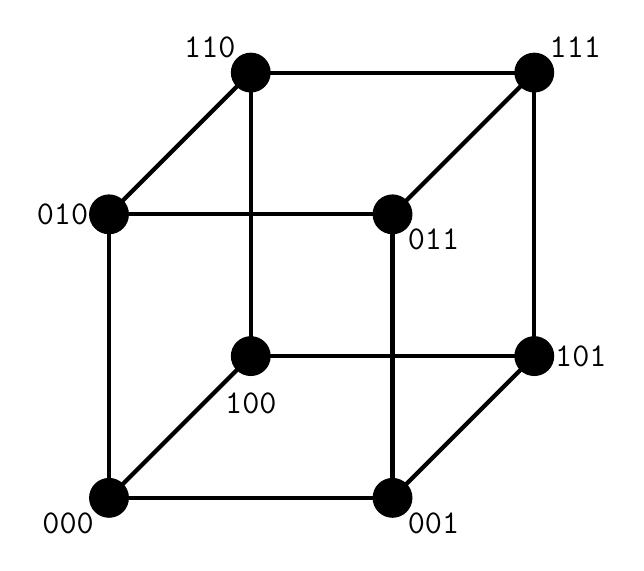
\begin{tikzpicture}[
    scale=1.2,
    vertex/.style={circle, draw=black, fill=black, minimum size=14pt, inner sep=0pt},
    edge/.style={draw=black, line width=1.5pt}
]
 
% Współrzędne wierzchołków sześcianu dla przedniej ściany
\coordinate (000) at (0,0);
\coordinate (001) at (3,0);
\coordinate (010) at (0,3);
\coordinate (011) at (3,3);
 
% Współrzędne wierzchołków sześcianu dla tylnej ściany
\coordinate (100) at (1.5,1.5);
\coordinate (101) at (4.5,1.5);
\coordinate (110) at (1.5,4.5);
\coordinate (111) at (4.5,4.5);
 
% Rysowanie krawędzi łączących przednią i tylną ścianę
\draw[edge] (000) -- (100);
\draw[edge] (001) -- (101);
\draw[edge] (010) -- (110);
\draw[edge] (011) -- (111);
 
% Rysowanie krawędzi tylnej ściany
\draw[edge] (100) -- (101) -- (111) -- (110) -- cycle;
 
% Rysowanie krawędzi przedniej ściany
\draw[edge] (000) -- (001) -- (011) -- (010) -- cycle;
 
% Rysowanie okrągłych węzłów w wyznaczonych punktach
\node[vertex] (n000) at (000) {};
\node[vertex] (n001) at (001) {};
\node[vertex] (n010) at (010) {};
\node[vertex] (n011) at (011) {};
\node[vertex] (n100) at (100) {};
\node[vertex] (n101) at (101) {};
\node[vertex] (n110) at (110) {};
\node[vertex] (n111) at (111) {};
 
% Dodawanie etykiet tekstowych opisujących poszczególne stany
\node[below left, font=\large, xshift=-2pt, yshift=-2pt] at (n000) {\texttt{000}};
\node[below right, font=\large, xshift=2pt, yshift=-2pt] at (n001) {\texttt{001}};
\node[left, font=\large, xshift=-4pt] at (n010) {\texttt{010}};
\node[below right, font=\large, xshift=2pt, yshift=-2pt] at (n011) {\texttt{011}};
\node[below, font=\large, yshift=-10pt] at (n100) {\texttt{100}};
\node[right, font=\large, xshift=4pt] at (n101) {\texttt{101}};
\node[above left, font=\large, xshift=-2pt, yshift=2pt] at (n110) {\texttt{110}};
\node[above right, font=\large, xshift=2pt, yshift=2pt] at (n111) {\texttt{111}};
 
\end{tikzpicture}
\caption{Graficzna reprezentacja odległości Hamminga w trójwymiarowej przestrzeni.}
\label{rys:hamming}
\end{figure}
 
W klasycznej teorii kodowania oraz systemach transmisji danych opisane podejście znajduje zastosowanie przy detekcji i korekcji błędów ze względu na wysoką efektywność w dyskretnych systemach cyfrowych, okazuje się jednak niewystarczające w problematyce modelowania ciągłych układów dynamicznych. W odniesieniu do ciągłych trajektorii fazowych drobne zaburzenie numeryczne nie reprezentuje odosobnionego przekłamania bitowego, lecz zmianę stanu początkowego, która podlega ewolucji czasowej. W związku z tym binarne miary odległości ustępują miejsca metodom statystycznym służącym do oceny korelacji zachodzących pomiędzy sygnałami. 
 
\section{Korelacja Pearsona i Spearmana}
Współczynnik korelacji liniowej Pearsona stanowi powszechnie stosowaną w statystyce miarę służącą do ilościowego określania poziomu oraz kierunku współzależności liniowej pomiędzy dwiema zmiennymi losowymi. Wskaźnik ten jest wyznaczany w celu weryfikacji hipotezy, czy zmianom wartości jednej zmiennej towarzyszą proporcjonalne zmiany wartości drugiej zmiennej.
 
Obliczenie współczynnika korelacji opiera się na podzieleniu kowariancji, stanowiącej miarę wspólnej zmienności, przez iloczyn odchyleń standardowych rozpatrywanych zmiennych~\cite{korelacjaPearsona1, korelacjaPearsona2}, co opisuje zależność:
\begin{equation}
r = \frac{\sum_{i=1}^{n} (x_i - \bar{x})(y_i - \bar{y})}{\sqrt{\sum_{i=1}^{n} (x_i - \bar{x})^2} \sqrt{\sum_{i=1}^{n} (y_i - \bar{y})^2}}
\label{eq:korelacja_pearsona}
\end{equation} 
 
gdzie:
\begin{itemize}
    \item $x_i$ oraz $y_i$ reprezentują poszczególne obserwacje uzyskane dla badanych zmiennych,
    \item $\bar{x}$ oraz $\bar{y}$ oznaczają średnie arytmetyczne wyznaczone dla analizowanych próbek,
    \item $n$ definiuje całkowitą liczność próby danych.
\end{itemize}
 
Wartość tego wskaźnika zawiera się w przedziale zamkniętym $[-1, 1]$, gdzie wynik dodatni wskazuje na współbieżność kierunków zmian obu zmiennych, natomiast wartość ujemna oznacza relację odwrotną, w której wzrostowi jednej wartości towarzyszy spadek drugiej. Bliskość wartości bezwzględnej współczynnika do jedności świadczy o silnej zależności liniowej, podczas gdy wartość równa zeru reprezentuje brak korelacji o charakterze liniowym~\cite{korelacjaPearsona3, korelacjaPearsona4}, co jednak nie wyklucza istnienia silnych powiązań o charakterze nieliniowym. Poprawna interpretacja i stosowanie tej metody wymaga wcześniejszej weryfikacji założeń dotyczących braku obserwacji odstających oraz zgodności rozkładów analizowanych parametrów z rozkładem normalnym.
 
Klasyczne metody statystyczne wykazują ograniczenia wynikające z możliwości identyfikacji jedynie liniowych zależności w strukturach danych. Ze względu na to, że współczynnik Pearsona nie opisuje związków nieliniowych, do analizy bardziej złożonych powiązań wykorzystuje się współczynnik korelacji rang Spearmana, umożliwiający wykrywanie monotonicznych trendów zmian bez konieczności spełnienia założenia o liniowości.
 
Procedura wyznaczania tego wskaźnika wymaga wstępnego uporządkowania zgromadzonych danych badawczych pod względem ich wartości oraz przypisania im odpowiednich rang, co umożliwia określenie różnic między rangami odpowiadających sobie obserwacji. Współczynnik korelacji rangowej oblicza się na podstawie następującej zależności matematycznej~\cite{spearman1}:
 
\begin{equation}
r_s = 1 - \frac{6 \sum_{i=1}^{n} d_i^2}{n(n^2 - 1)}
\label{eq:korelacja_spearmana}
\end{equation}
 
gdzie:
\begin{itemize}
    \item $d_i$ określa różnicę pomiędzy rangami przypisanymi odpowiednio obserwacjom $x_i$ oraz $y_i$,
    \item $n$ reprezentuje całkowitą liczbę par danych w próbie.
\end{itemize}
 
Analiza rangowa może okazać się niewystarczająca w przypadku struktur sygnałowych o wysokim stopniu złożoności, ponieważ procesy chaotyczne charakteryzują się głęboką nieliniowością, manifestującą się gwałtownymi fluktuacjami amplitudy oraz ciągłymi oscylacjami wokół wielowymiarowych trajektorii. W takich warunkach klasyczne wskaźniki statystyczne przyjmują wartości bliskie zeru, co prowadzi do błędnych wniosków o braku współzależności, podczas gdy badane sygnały pozostają ze sobą ściśle powiązane deterministycznie. Ograniczenia binarnej oceny odległości oraz tradycyjnych współczynników korelacji wymuszają wdrożenie specjalistycznych metod analitycznych w dziedzinie częstotliwości, obejmujących gęstość widmową mocy, a także miar bazujących na wykładnikach Lapunowa.
 
\section{Analiza w dziedzinie częstotliwości i widmo mocy}
 
Wobec faktu, iż złożoność i nieregularność sygnałów chaotycznych powodują, że analiza prowadzona wyłącznie w dziedzinie czasu okaze się niewystarczająca do pełnego opisu dynamiki układu~\cite{FFT1, FFT2}, standardowo stosuje się transformację sygnału do dziedziny częstotliwości. Umożliwia to identyfikację dominujących składowych harmonicznych oraz zbadanie rozkładu energii w systemie, a podstawowym narzędziem realizującym to zadanie jest dyskretna transformata Fouriera (ang. \textit{Discrete Fourier Transform}, DFT).
 
Dla dyskretnego szeregu czasowego składającego się z $N$ próbek $x_n$, transformatę Fouriera $X_k$ definiuje równanie:
 
\begin{equation}
X_k = \sum_{n=0}^{N-1} x_n e^{-i \frac{2\pi}{N} k n}
\label{eq:dft_v2}
\end{equation}
gdzie:
\begin{itemize}
   \item $X_k$ określa wyznaczoną wartość dla $k$-tego prążka widma częstotliwościowego analizowanego sygnału,
   \item $x_n$ definiuje wartość $n$-tej próbki rozpatrywanego sygnału w dziedzinie czasu,
   \item $N$ reprezentuje całkowitą liczbę próbek sygnału zgromadzonych w poddanej analizie próbie badawczej,
   \item $k$ oznacza indeks kolejnych prążków częstotliwościowych, który przyjmuje wartości ze zbioru $0, 1, \dots, N-1$,
   \item $n$ stanowi indeks kolejnych próbek dyskretnych w dziedzinie czasu,
   \item $i$ to jednostka urojona.
\end{itemize}
 
Wynik transformacji dostarcza informacji o amplitudzie i fazie poszczególnych składowych, jednak w analizie zjawisk chaotycznych kluczowe znaczenie ma gęstość widmowa mocy, pozwalająca na określenie sposobu rozkładu mocy sygnału w funkcji częstotliwości. Ze względu na to, że zespolone współczynniki $X_k$ dla sygnałów rzeczywistych wykazują symetrię sprzężoną, w analizie uwzględnia się wyłącznie pierwszą połowę widma, aż do częstotliwości Nyquista ($k \le N/2$). Wartość widma mocy $P_k$ dla danej częstotliwości oblicza się jako kwadrat modułu zespolonego współczynnika Fouriera:
 
\begin{equation}
P_k = |X_k|^2 = \operatorname{Re}(X_k)^2 + \operatorname{Im}(X_k)^2
\label{eq:widmo_mocy_v2}
\end{equation}
 
Sygnały deterministycznie chaotyczne charakteryzują się specyficznym, szerokopasmowym widmem mocy, które w przeciwieństwie do układów okresowych o widmie złożonym z pojedynczych, ostrych prążków oraz w opozycji do czystego szumu o płaskim rozkładzie, zawiera zazwyczaj ciągłe, opadające tło szumowe z wyraźnie zaznaczonymi częstotliwościami podstawowymi. Wykresy widma mocy powszechnie prezentuje się w skali półlogarytmicznej z logarytmiczną osią rzędnych, co umożliwia jednoczesną obserwację składowych o skrajnie zróżnicowanym poziomie energii.
 
\section{Wykładnik Lapunowa}
 
Pojęcie wykładnika Lapunowa zostało sformułowane w 1892 roku przez rosyjskiego uczonego Aleksandra Michajłowicza Lapunowa w rozprawie doktorskiej pod tytułem \textit{„The general problem of the stability of motion”}~\cite{lyapunov1992}. Badania były ukierunkowane na poszukiwanie matematycznych metod pozwalających na precyzyjne określenie stabilności układów nieliniowych, co doprowadziło do zdefiniowania tak zwanych liczb charakterystycznych, znanych dziś powszechnie jako wykładniki Lapunowa~\cite{wykładnikLaponowa1, wykładnikLaponowa2}.
 
Wykładnik Lapunowa pozwala ocenić tempo, w jakim dwie początkowo bliskie sobie trajektorie zbliżają się do siebie lub oddalają w przestrzeni czasu~\cite{wykładnikLaponowa3, wykładnikLaponowa4}. Dodatni największy wykładnik Lapunowa (ang. \textit{Largest Lyapunov Exponent}, LLE) wskazuje na obecność chaosu, ponieważ oznacza, że trajektorie oddalają się od siebie w sposób wykładniczy, które to zjawisko opisywane jest wzorem:
 
\begin{equation}
\Delta_k \approx \Delta_0 e^{\lambda_{\max} k}
\end{equation}
 
gdzie:
\begin{itemize}
    \item $\lambda_{\max}$ to największy wykładnik Lapunowa,
    \item $\Delta_0$ to odległość początkowa między trajektoriami,
    \item $\Delta_k$ to odległość między trajektoriami po $k$ krokach czasowych.
\end{itemize}
Zależność przedstawiono schematycznie na rysunku~\ref{fig:wykladnik_schemat}.
 
\begin{figure}[htbp]
    \centering
    \begin{tikzpicture}
        % Odległość początkowa
        \node at (0, 1.0) {Odległość między dwiema wartościami początkowymi:};
        \draw (-1.5,0) -- (1.5,0);
        \draw (-1.5,-0.1) -- (-1.5,0.1);
        \draw (1.5,-0.1) -- (1.5,0.1);
        \node[above] at (0,0) {$\varepsilon$};
        \node[below] at (-1.5,-0.1) {$x_0$};
        \node[below] at (1.5,-0.1) {$x_0 + \varepsilon$};
        
        % Po N iteracjach (zmniejszony odstęp, y z -2 na -1.2)
        \node at (0, -1.2) {Po $N$ iteracjach:};
        
        % Dolna oś (podniesiona z y=-3.5 na y=-2.2)
        \draw (-2.5,-2.2) -- (2.5,-2.2);
        \draw (-2.5,-2.3) -- (-2.5,-2.1);
        \draw (2.5,-2.3) -- (2.5,-2.1);
        \node[above] at (0,-2.2) {$\varepsilon e^{N\lambda(x_0)}$};
        \node[below] at (-2.5,-2.3) {$f^N(x_0)$};
        \node[below] at (2.5,-2.3) {$f^N(x_0 + \varepsilon)$};
    \end{tikzpicture}
    \caption{Wizualizacja dywergencji początkowych trajektorii}
    \label{fig:wykladnik_schemat}
\end{figure}
 
W rzeczywistych układach fizycznych przyjmuje się założenie, że trajektorie nie mogą oddalić się od siebie bardziej, niż wynosi całkowity rozmiar atraktora, w którym są uwięzione, w związku z czym powyższe równanie ma zastosowanie wyłącznie dla małych wartości $k$, odpowiadających początkowej fazie ewolucji układu. Po zlogarytmowaniu obu stron uzyskuje się liniowe równanie prostej:
 
\begin{equation}
\ln \Delta_k = \ln \Delta_0 + k \lambda_{\max}
\end{equation}
 
Największy wykładnik Lapunowa stanowi zatem współczynnik kierunkowy prostej dopasowanej do opisanego równania~\cite{wykładnikLaponowa5, wykładnikLaponowa6}. 
 
\subsection{Algorytm Rosensteina}
 
W praktyce numerycznej do szacowania wartości największego wykładnika Lapunowa na podstawie skończonych szeregów czasowych powszechnie stosuje się algorytm Rosensteina~\cite{rosenstein1993}. Podejście to zakłada, że dla wybranego punktu referencyjnego na trajektorii wyszukuje się najbliższego sąsiada w przestrzeni, a następnie bada się, w jaki sposób odległość między nimi ($d_j$) rośnie w kolejnych dyskretnych krokach czasowych, co opisuje funkcja:
 
\[d_j(k)\approx C_j e^{\lambda_1 k\Delta t}\]
 
Po zlogarytmowaniu obu stron otrzymuje się zależność liniową:
 
\[\ln(d_j(k))\approx\ln(C_j)+\lambda_1 k\Delta t\]
 
Aby uśrednić zakłócenia występujące w danych, oblicza się średnią po wielu zidentyfikowanych parach sąsiadów $M$:
 
\[y(k)=\frac{1}{M}\sum_{j=1}^M\ln(d_j(k))\approx\lambda_1 k\Delta t+C\]
 
Największy wykładnik Lapunowa $\lambda_1$ określa się ostatecznie jako nachylenie prostej dopasowanej do wykresu średniego tempa oddalania się punktów $y(k)$ w funkcji czasu~\cite{rosensteina}.
 
\section{Modelowanie zjawisk chaotycznych za pomocą sztucznych sieci neuronowych GAN}
 
Modelowanie układów charakteryzujących się wysokim stopniem nieliniowości oraz wrażliwością na parametry początkowe wymaga zastosowania zaawansowanych aparatów obliczeniowych, do których zalicza się sztuczne sieci neuronowe. Metody te wykazują znaczną skuteczność z uwagi na zdolność do aproksymacji złożonych funkcji nieliniowych, a biorąc pod uwagę fakt, że zjawiska chaotyczne są trudne do analitycznego opisania klasycznymi równaniami, uzasadnienie znajduje wdrożenie nowoczesnych podejść algorytmicznych do ich numerycznej generacji. Do realizacji tego celu stosowana jest architektura generatywnych sieci przeciwstawnych (ang. \textit{Generative Adversarial Networks}, GAN), umożliwiająca odtwarzanie złożonych trajektorii fazowych na podstawie ekstrakcji ukrytych zależności i powtarzalnych wzorców dynamicznych układu.
 
Koncepcja generatywnych sieci przeciwstawnych została przedstawiona w 2014 roku w pracy „Generative Adversarial Nets”~\cite{goodfellow2014generative} jako rezultat badań prowadzonych na Uniwersytecie w Montrealu. Architektura GAN opiera się na integracji dwóch współpracujących i jednocześnie konkurujących ze sobą modeli strukturalnych: generatora oraz dyskryminatora, których wzajemne powiązania zilustrowano na rysunku~\ref{rys:GAN_wynik}.

\begin{figure}[h!]
\centering 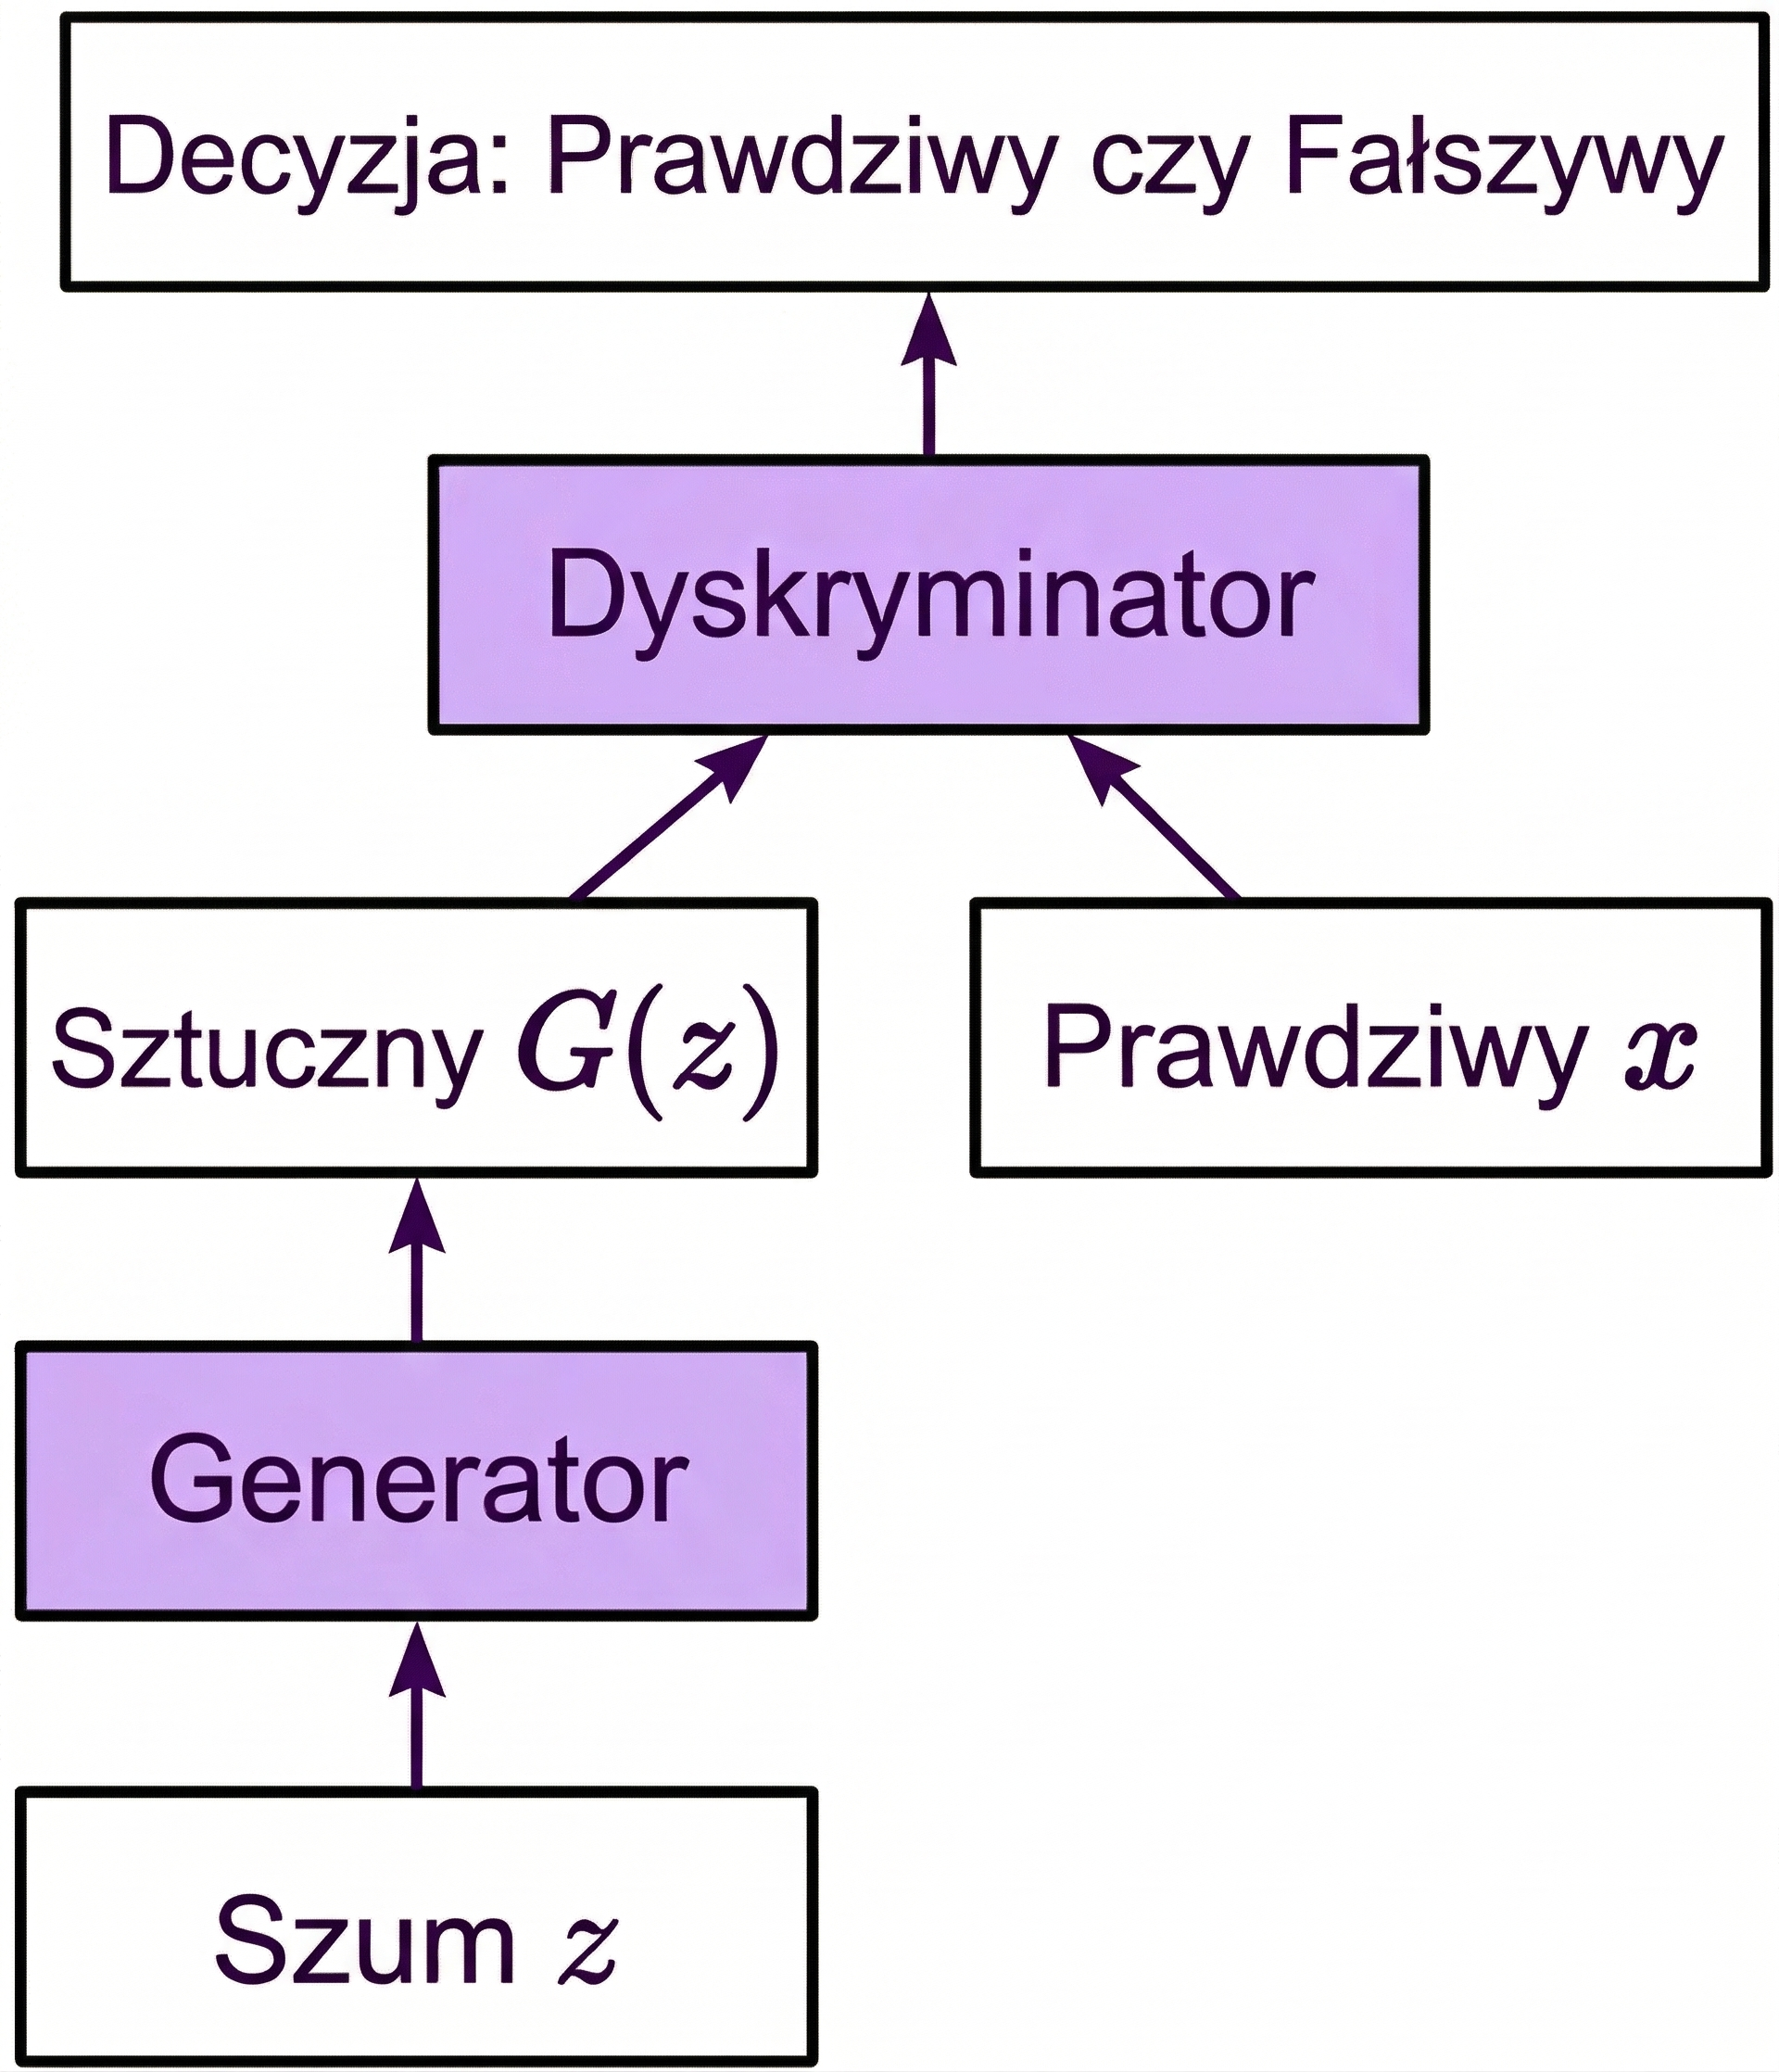
\includegraphics[width=0.45\linewidth]{rysunki/GAN.png}
\caption{Schemat blokowy i przepływ danych w sieci GAN} 
\label{rys:GAN_wynik}
\end{figure}

Proces optymalizacji tych podsieci odzwierciedla założenia teorii gier o sumie zerowej, gdzie rozwój jednego z modeli stymuluje adaptację drugiego, co wymusza ciągłą aktualizację wag synaptycznych w kolejnych epokach treningowych~\cite{goodfellow2019, goodfellow2020}. 
 
W ujęciu formalnym proces ten jest definiowany jako problem optymalizacji typu minimaks, realizowany za pomocą funkcji wartości $V(D, G)$:
 
\begin{equation} 
\min_G \max_D V(D, G) = \mathbb{E}_{x \sim p_{\mathrm{data}}(x)} [\log D(x)] + \mathbb{E}_{z \sim p_z(z)} [\log(1 - D(G(z)))] 
\label{eq:gan_minimax}
\end{equation}
 
gdzie:
\begin{itemize}
    \item zmienna $x$ odzwierciedla próbki pochodzące z rzeczywistego rozkładu danych,
    \item zmienna $z$ oznacza wektor wejściowego szumu losowego,
    \item wyrażenie $G(z)$ reprezentuje syntetyczny sygnał wytworzony przez generator,
    \item wyrażenie $D(x)$ określa prawdopodobieństwo przypisania badanej próbki do zbioru danych rzeczywistych przez dyskryminator.
\end{itemize}
 
Funkcja generatora polega na syntezie nowych, realistycznych danych, przy czym nadrzędnym celem w kontekście szeregów czasowych staje się predykcja kolejnych punktów trajektorii. Wprowadzenie szumu losowego o niskiej amplitudzie na etapie początkowym zapobiega powstawaniu powtarzalnych wzorców i zapewnia wymaganą wariancję generowanych przebiegów, a optymalizacja parametrów zmierza do zminimalizowania zdolności dyskryminatora do odróżnienia danych syntetycznych od rzeczywistych~\cite{goodfellow2016, GAN}.
 
Z kolei dyskryminator pełni rolę weryfikacyjną, przetwarzając naprzemiennie sekwencje sygnałów rzeczywistych oraz syntetycznych w celu ich poprawnej klasyfikacji pod kątem autentyczności. W trakcie procedury treningowej oba układy równolegle modyfikują swoje parametry wewnętrzne, co prowadzi do sukcesywnego wzrostu efektywności całego systemu przeciwstawnego.
 
Poprawnie przeprowadzony proces uczenia prowadzi do osiągnięcia stanu równowagi, w którym generator tworzy próbki o statystyce identycznej z danymi rzeczywistymi, natomiast dyskryminator traci zdolność różnicowania pochodzenia sygnałów, co sprowadza prawdopodobieństwo poprawnej klasyfikacji do wartości 0.5, odpowiadającej losowemu wyborowi.
 
\section{Sieci z pamięcią LSTM}
 
Konwencjonalne architektury sieci neuronowych wykazują ograniczenia podczas przetwarzania długich sekwencji czasowych, wynikające bezpośrednio z braku struktur pamięciowych, co prowadzi do utraty informacji o początkowych stanach sygnału wskutek zjawiska zanikania gradientu. Zagadnienie to zostało rozwiązane poprzez wprowadzenie architektury LSTM (ang. \textit{Long Short-Term Memory}) przez Seppa Hochreitera i Jürgena Schmidhubera w 1997 roku~\cite{hochreiter1997long}, implementującej zaawansowane mechanizmy kontroli przepływu informacji w dziedzinie czasu. Wspomniane rozwiązanie bywa współcześnie integrowane z modelami klasy GAN w celu istotnego podniesienia dokładności odwzorowania ciągłych oraz wysoce nieliniowych przebiegów dynamicznych~\cite{GANLSTM1, GANLSTM2, GANLSTM3}.
 
Opisywane możliwości modelowania wynikają bezpośrednio z wewnętrznej budowy sieci, w której podstawą działania pojedynczej komórki jest stan wewnętrzny $C_t$. Stan ten pełni funkcję głównego toru informacyjnego, co umożliwia przenoszenie ważnych cech sygnału przez kolejne etapy obliczeniowe bez utraty danych z początkowych kroków~\cite{LSTM1}. Zarządzanie procesem zapisu i odczytu danych odbywa się za pomocą struktur zwanych bramkami, które wykorzystują operacje macierzowe oraz nieliniowe funkcje aktywacji, takie jak funkcja sigmoidalna $\sigma$ i tangens hiperboliczny $\tanh$, do dokładnego filtrowania przepływających strumieni informacji, a cały ten proces matematyczny wewnątrz komórki przedstawiono na rysunku~\ref{rys:LSTM_schemat}.

 
\begin{figure}[h!]
\centering
\usetikzlibrary{positioning}
\begin{tikzpicture}[
    node distance=1.5cm and 1cm,
    data/.style={draw, very thick, fill=white, minimum width=3.8cm, minimum height=1.2cm, align=center, font=\large},
    process/.style={draw, very thick, fill=purple!30, minimum width=4.5cm, minimum height=1.2cm, align=center, font=\large},
    arrow/.style={-stealth, very thick}
]
 
% Dane wejściowe na samym dole
\node[data] (xt) {Dane wejściowe $x_t$};
\node[data, right=1cm of xt] (ht1) {Poprzedni stan\\ukryty $h_{t-1}$};
 
% Bramki filtrujące dane
\coordinate (srodek_dol) at ($(xt.north)!0.5!(ht1.north)$);
\node[process, above=1.2cm of srodek_dol] (bramki) {Bramy informacyjne\\(zapominania $f_t$ i wejściowa $i_t$)};
 
% Główna aktualizacja stanu komórki
\node[process, above=1.5cm of bramki] (update) {Aktualizacja stanu komórki\\$C_t = f_t \cdot C_{1} + i_t \cdot \tilde{C}_t$};
\node[data, left=1cm of update] (ct1) {Poprzedni stan\\pamięci $C_{t-1}$};
 
% Brama wyjściowa generująca końcowy wynik
\node[process, above=1.5cm of update] (wyjscie) {Brama wyjściowa\\$h_t = o_t \cdot \tanh(C_t)$};
 
% Ostateczne wyniki na górze wykresu
\node[data, above=1.5cm of wyjscie] (ht) {Nowy stan ukryty $h_t$};
\node[data, right=1.5cm of ht] (ct) {Nowy stan pamięci $C_t$};
 
% Rysowanie strzałek łączących poszczególne bloki
\draw[arrow] (xt.north) -- (bramki.south -| xt.north);
\draw[arrow] (ht1.north) -- (bramki.south -| ht1.north);
 
\draw[arrow] (bramki.north) -- (update.south);
\draw[arrow] (ct1.east) -- (update.west);
 
\draw[arrow] (update.north) -- (wyjscie.south);
 
\draw[arrow] (wyjscie.north) -- (ht.south);
\draw[arrow] (update.east) -| (ct.south) node[pos=0.25, above, font=\large] {Pamięć $C_t$};
 
\end{tikzpicture}
\caption{Schemat blokowy komórki pamięci LSTM obrazujący matematyczny przepływ informacji.}
\label{rys:LSTM_schemat}
\end{figure}
 
Sekwencję przetwarzania danych wewnątrz pojedynczego bloku pamięciowego można podzielić na cztery powiązane ze sobą etapy decyzyjne. W fazie pierwszej brama zapominania dokonuje ewaluacji przydatności dotychczasowych informacji, decydując o stopniu usunięcia z pamięci składowych, które utraciły znaczenie dla predykcji:
 
\begin{equation}
    f_t = \sigma(W_f \cdot [h_{t-1}, x_t] + b_f)
\end{equation}
 
W kolejnym kroku brama wejściowa analizuje bieżący wektor danych $x_t$, przypisując mu odpowiednie wagi synaptyczne i formując wektor kandydujący nowych wartości przeznaczonych do zapisu w stanie pamięci komórki:
 
\begin{equation}
    i_t = \sigma(W_i \cdot [h_{t-1}, x_t] + b_i)
\end{equation}
\begin{equation}
    \tilde{C}_t = \tanh(W_C \cdot [h_{t-1}, x_t] + b_C)
\end{equation}
 
Na podstawie wyznaczonych stanów aktywacji obu bram realizowana jest właściwa aktualizacja stanu pamięci komórki, podczas której zachowane składowe historyczne są integrowane z nowo wyekstrahowanymi cechami sygnału wejściowego:
 
\begin{equation}
    C_t = f_t \cdot C_{t-1} + i_t \cdot \tilde{C}_t
\end{equation}
 
Proces przetwarzania kończy się w obszarze bramy wyjściowej, która na bazie zaktualizowanego i przefiltrowanego stanu wewnętrznego generuje wektor wyjściowy warstwy, przekazując jednocześnie stan ukryty $h_t$ do następnego kroku dyskretnego w celu zachowania ciągłości symulacji:
 
\begin{equation}
    o_t = \sigma(W_o \cdot [h_{t-1}, x_t] + b_o)
\end{equation}
\begin{equation}
    h_t = o_t \cdot \tanh(C_t)
\end{equation}
 
W złożonych modelach generatywnych struktury rekurencyjne bywają poprzedzane jednowymiarowymi warstwami splotowymi (Conv1D), realizującymi zadanie wstępnej filtracji sygnału wejściowego, co odciąża główne moduły pamięciowe. Operacja przesuwania jądra splotu nad surowym szeregiem czasowym umożliwia efektywną ekstrakcję lokalnych wzorców dynamicznych, takich jak nagłe zmiany amplitudy, zapewniając jednocześnie redukcję komponentu szumowego przed wprowadzeniem danych do właściwej analizy sekwencyjnej~\cite{goodfellow2016deep, Conv1DLSTM2, Conv1DLSTM}.



















